\section{3D-Laplace}
The previous sub-section described the use of 2-dimensional noise on geographical data.
This approach has recently been extended to support 3-dimensional data, which benefits indoor navigation \citep{9646489}.
The method is similar to the 2D approach but includes the azimuth angle $\psi$ besides the polar angle $\theta$ and radial distance $r$.

\subsection{Geo-indistinguishability}
To establish the same privacy guarantees for 3-dimensional data as for 2-dimensional data, the original equation \ref{algo:2d-geo-indistinguishability} is extended \citep{9646489}.
\begin{equation}
  K(x_1)(z) \le e^{\epsilon * d_3(x_1, x_2)} K(x_2)(z)
  \label{algo:3d-geo-indistinguishability}
\end{equation}
Where $x_1$ and $x_2$ are two real data points in the same dataset $X$, and $K$ is the probability.
%The more $x_1$ and $x_2$ are similar, the more the perturbed location distributions $K(x_1)(z)$ and $K(x_2)(z)$ need to be similar.
\subsection{Spherical Laplace}
Implementing the 3D-Laplace is based on the same method as the 2D-Laplace mechanism.
Therefore, the \gls{pdf} where the noise is drawn from is almost identical \citep{9646489}:
\begin{equation}
  D_{\epsilon}(x_i)(x_0) = A \cdot e^{-\epsilon \cdot d_3(x_i, x_0)}
  \label{eq:3d-laplace-pdf}
\end{equation}
Where $A$ is the normalization factor, and $d_3$ is the Euclidean distance in a 3-dimensional space.
Instead of only consisting of a polar angle $\theta$ and radial distance $r$, the third dimension (altitude) is the azimuth angle $\psi$ \citep{9646489}:
\begin{equation}
  D_{\epsilon}(x_i)(x_0) = \frac{1}{4 \cdot \pi^2} \cdot \epsilon^3 \cdot r^2 \cdot e^{-\epsilon \cdot r}
  \label{eq:3d-laplace-with-normalization}
\end{equation}
The distance between $x_i$ and $x_0$ is replaced by $r$, leaving us with the normalization factor.
As with the 2D-Laplace, we are most interested in the normalization factor, which uses the three coordinates \citep{9646489}.
Because these can be sampled independently, Min et al. formulate three marginal distributions $D$ for each coordinate: $R$, $\Theta$ and $\Psi$ \citep{9646489}:
%The implementation of Min et al. projects the dimensions onto a sphere instead of a circle \citep{9646489}.
%This sphere is a unit sphere calculated with a radius of 1. \newline
%\textbf{Calculating $\theta$ and $\psi$}: The tuple $U = (\theta, \psi)$ is randomly drawn from the unit sphere using the following equations \citep{9646489}:
\begin{subequations}

  \begin{align}
     & D_\epsilon, R(r) = \frac{1}{2} \epsilon^3 \cdot r^2 \cdot e^{-\epsilon \cdot r} \label{eq:3d-laplace-1} \\
     & D_\epsilon, \Theta(\theta) = \frac{1}{\pi}                                      \label{eq:3d-laplace-2} \\
     & D_\epsilon, \Psi(\psi) = \frac{1}{2 \cdot \pi} \label{eq:3d-laplace-3}
  \end{align}
\end{subequations}
\begin{itemize}
  \item The radius $r$ is sampled randomly from the Gamma distribution (Equation \ref{eq:3d-laplace-1}) with a shape of 3 and a scale of $1/\epsilon$ \citep{9646489}.
  \item The $\theta$ and $psi$ are also random sampled from the uniform distribution with the range given in Equations \ref{eq:3d-laplace-2} and \ref{eq:3d-laplace-3} \citep{9646489}.
\end{itemize}
Finally, the noise is added to the original location $x$ to obtain the perturbed location $z = x + U*r$ (See Figure \ref{fig:3d-laplace-noise}).
The spherical coordinates $(r, \theta, \psi)$ are converted to the Cartesian coordinates $(x, y, z)$ to obtain the perturbed location $z$:
\begin{align*}
  z_x = r * \sin(\theta) * \sin(\psi) \\
  z_y = r * \sin(\theta) * \cos(\psi) \\
  z_z = r * \cos(\theta)
\end{align*}
The complete overview is visualized in figure \ref{fig:3d-laplace}.
\begin{figure}[H]
  \includesvg[width=1\textwidth]{TheorethicalFramework/ND-Laplace/Images/3d_laplace.svg}
  \caption{3D-Laplace noise distribution according to the method proposed by Min et al. \citep{9646489}}
  \label{fig:3d-laplace}
\end{figure}
The above figure shows the whole process of generating noise for a single point $x_0$ (left) to a new point $z$ (right).
As observed, the noise is generated using a sphere and converted to a cartesian coordinate system.
\newpage
\begin{figure}[H]
  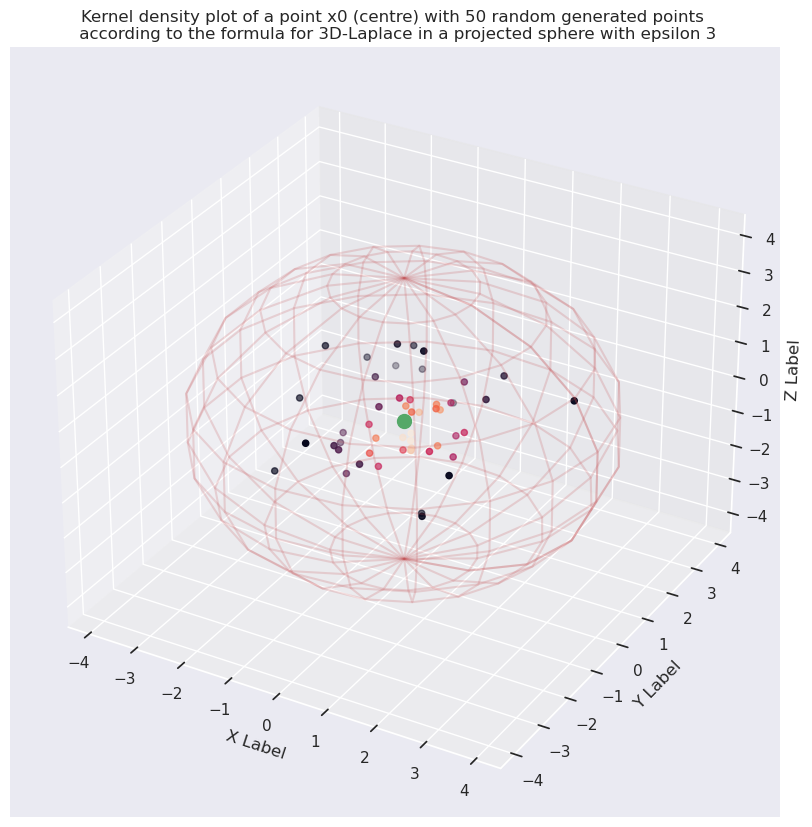
\includegraphics[width=0.6\textwidth]{TheorethicalFramework/ND-Laplace/Images/3d_laplace_noise.png}
  \caption{50 random noise samples generated around point $x_0$ (green dot) using the 3D-Laplace noise method \citep{9646489} plotted on a sphere.}
  \label{fig:3d-laplace-noise}
\end{figure}
This figure shows an example of the noise generated around a point $x_0$ (green dot).
For this purpose, 50 random samples were generated using the 3D-Laplace noise method.
As is visible, most points are plotted close to $x_0$ and fewer at the sphere's surface, according to the Gaussian distribution.

\newpage
\subsection{Truncation}
As with the 2D-Laplace method, the 3D-Laplace method also needs a discretization method that is used to truncate the data.
Instead of a plane grid $G$, Min et al. extended this to a cuboid grid $G_c$ to support 3-dimensional data \citep{9646489}.
This impacts the probability $K$, as was the case with the 2D-Laplace method (See Equation: \ref{eq:grib-probability}).
The equation is extended by Min et al. to support 3-dimensional data \citep{9646489}:
\begin{equation}
  N(x_0) = { y \in R^3 | \forall'_{0} \in G_c \cdot d_3(x'_{0}, y) \leq d_3(x_0, y)}
  \label{eq:3d-grid-probability}
\end{equation}
So, the complete probability for a point $x_0$ being generated by the 3D-Laplace method to be part of $G_c$ is:
\begin{equation}
  N_B(x_0) = N(x_0) \cap Z
  \label{eq:3d-grid-probability-2}
\end{equation}
Here, $Z$ is the discrete set of points of $X$ generated according to the 3D-Laplace mechanism.
According to the mechanism, $Z$ depends on the radial distance $r$, but now also needs to consider $G_c$.
The latter stays the same size, while the radius $r$ differs according to \ref{eq:3d-laplace-1}.
This jeopardizes geo-indistinguishability, and therefore Min et al. provided a modified version of Theorem \ref{theorem:discretization} \citep{9646489}.
Moreover, they extend the original theorem (See Theorem \ref{theorem:discretization}) to support 3-dimensional data.
They define the cuboid $G_c$ using the units $u, w, h$ (length, width, and height).
Now these are established, we provide the extended theorem as provided by Min et al. to show \gls{gi} holds for the maximum radius of $r_M$ \citep{9646489}:
\begin{theorem}
  Assume $R_M < \frac{w}{d_0}, d_r \leq \frac{r_M \cdot d_\theta \cdot h}{w}$, and let \\
  $w = \frac{u \cdot w}{r^2_M \cdot sin \cdot \theta \cdot d_\psi \cdot d_\theta} > \frac{v}{r_M \cdot d_\psi}$. Let $\epsilon, \epsilon' \in R^+$ such that \\
  $\epsilon' + \frac{1}{h} ln \frac{w + 3 \cdot e^{\epsilon' \cdot h}}{w - 3 \cdot e^{\epsilon' \cdot h}} \leq \epsilon$ \\
  Then $K_{\epsilon'}$ satisfies $\epsilon$-geo-indistinguishability within the range \\
  of $r_M$. That is to say, if $d_3(x1, x')$ and $d_3(x_2, x') \leq r_M$ then, \\
  $K_{\epsilon'}(x_1)(x') \leq e^\epsilon \cdot d_3(x_1, x_2) \cdot K_{\epsilon'}(x_2)(x')$
  \label{theorem:3d-discretization}
\end{theorem}
This theorem is slightly longer than the 2-dimensional variant, but the principle stays the same.
\begin{enumerate}
  \item The device precision variables are defined as $d_0, d_\theta$, and $d_\psi$. Which is the hardware precision of the GPS-location or indoor navigation software.  Again, we omit this for the research; but nonetheless provide the full theorem.
  \item The cuboid $G_c$ is defined using the units $u, w, h$ (length, width, and height). The $h$ was used for the theorem as minimum grid-unit value, assuming that $u > v > h$ holds \citep{9646489}.
  \item Finally, the values $x_1, x_2$ should be lower or equal to the maximum radius $r_M$.
\end{enumerate}
%\todo[inline]{Maybe explain that we use the root of the function $f(x) = 0$ for the minimum value $h$ (height)}

We plotted example data points on a 3-dimensional grid in Figure \ref{fig:3d-laplace-example} to demonstrate this:
\begin{figure} [H]
  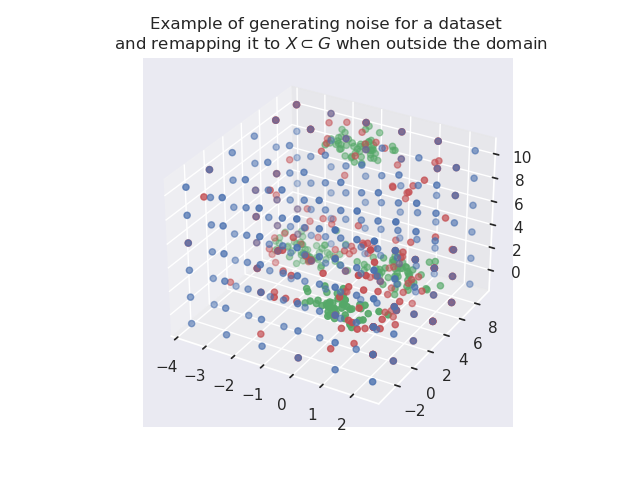
\includegraphics[width=\textwidth]{TheorethicalFramework/ND-Laplace/Images/example_3d_laplace.png}
  \caption{Applying 3-dimensional noise with $\epsilon = 1$ (red dots) to a dataset $X$ (green dots). Demonstrating remapping to the closest grid point (blue) or $X$.}
  \label{fig:3d-laplace-example}
\end{figure}

\newpage
\subsection{Final mechanism}
Finally, we provide as means of a summary the final algorithm for the Laplace mechanism for 3D space
\begin{algorithm}[H]
  \caption{Full algorithm for perturbing training data for 3D-clustering using planar/2D-Laplace \citep{DBLP:journals/corr/abs-1212-1984}}\label{alg:rq1}
  \begin{algorithmic}
    \Require $x \in X$  \Comment 3D array of points
    \Require $l \in R^ +$
    \Require $r \in R^ +$
    \Ensure $z \in Z$ \Comment 3D array of perturbed points
    %\State $r = \frac{\sigma}{2}$ \Comment formula 4.1
    \State $\epsilon \gets \frac{l}{r}$ \Comment Calculating privacy budget \citep{DBLP:journals/corr/abs-1212-1984}
    \State $Z \gets []$
    \For{$point_i \in X$}
    \State $\theta \gets [1, \pi2]$       \Comment Random noise according to equation \ref{eq:3d-laplace-1}.
    \State $p \gets \frac{1}{2\pi}$     \Comment Random noise according to equation \ref{eq:3d-laplace-2}.
    \State $r \gets \frac{1}{2}\epsilon^3 * r^2 * e^{-\epsilon * r}$          \Comment Draw $r$ based on equation \ref{eq:3d-laplace-3}
    %\State $z_i \gets T(x_{min}, x_{max}, point_i, z_i)$ \Comment algorithm 1.
    \State $z_x \gets r * \sin(\theta) * \sin(\psi)$
    \State $z_y \gets r * \sin(\theta) * \cos(\psi)$
    \State $z_z \gets r * \cos(\theta)$
    \State $Z::Add(z)$                      \Comment Adds z to the list Z.
    \EndFor
    \State \Return Z
  \end{algorithmic}
  \label{alg:3d-laplace}
\end{algorithm}
\newpage